\documentclass{article}
\usepackage{amsmath}
\usepackage{geometry}
\usepackage{graphicx}
\usepackage[hidelinks]{hyperref}
\usepackage[utf8]{inputenc}
\usepackage{minted} 

\title{Rekursion i Raytracing}
\author{Sebastian Bech Rasmussen}
\date{\today}

\begin{document}

% Title
\begin{titlepage}
    \maketitle
    \centering
    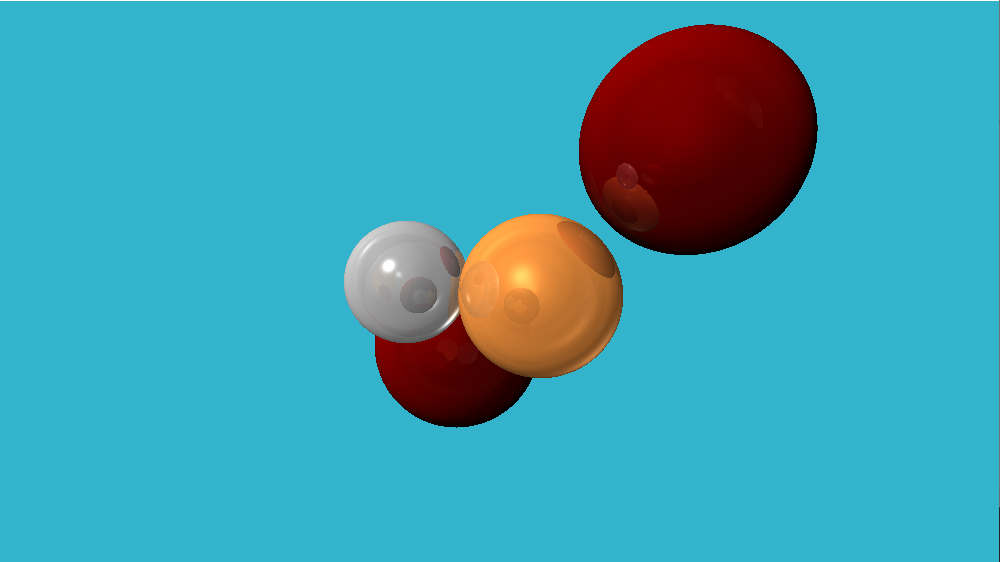
\includegraphics[scale=0.425]{images/raytracer.png}
\end{titlepage}

\tableofcontents

\newpage

\begin{flushleft}
    \section{Introduktion}

    Jeg synes det er super spændende, hvordan firmaer som Disney, Lucasarts og
    spilfirmaer som Electronic Arts eller Ubisoft kan skabe verdener, der virker så livagtige,
    at det næsten er som om vi var i dem selv, fysisk. Derfra fandt jeg hurtigt Raytracing,
    en teknik, der modellerer en 3D verden ud fra hvordan lys opfører sig.
    Tidligere har Raytracing kun været brugt i film, men med Nvidias RTX-grafikkort,
    virker raytracing nu også i realtime.
    I denne opgave undersøges sammenspillet mellem matematik og programmering med udgangspunkt i raytracing.

    \section{Problemstilling}

    \begin{enumerate}
        \item Hvad er raytracing?
        \item Hvorfor er raytracing bedre end andre grafik teknikker?
        \item Hvordan kan computerprogrammering forklare hvorfor raytracing er så tung en operation?
        \item Kan matematik bruges til at modellere en realistisk 3D verden?
    \end{enumerate}

    \section{Teori}

    I dette afsnit diskuteres relevant teori for henholdsvis matematik og programmering.

    \subsection{Matematik}

    \subsubsection{Talfølger}

    Talfølger er en følge eller liste af tal. Hver individuelle værdier i følgen kaldes for elementer.
    I nedenstående eksempel er det første element 2, og det andet 4 osv. De sidste 3 prikker betyder at talfølgen er uendelig
    \footnote{Rekursion \url{https://mathtxa.systime.dk/index.php?id=498&L=0}}.

    \[{a} = {2, 4, 6, 8, 10, ...}\]

    Derudover kan man referere til forskellige indekser ind i sin talfølge ved at bruge et tælletal:

    \[a_1 = 2\]
    \[a_2 = 4\]
    \[a_3 = 6\]

    Talfølger med den samme længde, altså samme antal elementer
    kan kombineres ved at addere eller subtraheres\footnote{Talfølger \url{https://mathtxa.systime.dk/?id=c2411&L=0}}.

    Talfølger kan også multipliceres med et tal:

    \[{a} = {1, 2, 3, 4}\]
    \[{a} \cdot 5 = {5, 10, 15, 20}\]

    \subsubsection{Rekursionsligninger}

    En rekursionsligning beregner en værdi med afsæt i en tidligere beregning.
    Løsningen til en rekursionsligning er en eller flere talfølger.
    En rekursionsligning er en form for regel, der beskriver hvordan et af elementerne i en talfølge skal beregnes.
    Dette betyder altså at alle elementer i talfølgen skal overholde rekursionsligningen
    \footnote{Rekursion \url{https://mathtxa.systime.dk/index.php?id=498&L=0}}.

    \subsubsection{Andengradsligninger}

    Det generelle andengradsligning er defineres således:

    \[ ax^2+bx+c = 0 \ \textrm{, for} \ a \neq 0\]

    En andengradsligning kan løses vha. af diskriminantformlen som lyder følgende
    \footnote{Diskriminantformlen, \url{https://www.webmatematik.dk/lektioner/matematik-b/andengradspolynomium-og-ligning/diskriminantformlen}}:

    \[D=b^2-4ac\]

    \begin{itemize}
        \item Hvis D er mindre end 0, har den ingen løsninger.
        \item Hvis D er 0, har den 1 løsning.
        \item Hvis D er større end 0, har den 2 løsninger.
    \end{itemize}

    Diskriminanten indsættes derefter i følgende for at finde løsningen, hvis den altså har en løsning:

    \[x = \frac{-b \pm \sqrt{D}}{2a}\]

    \subsubsection{Vektorer}

    En vektor er et objekt, der er defineret ved at have en længde og retning.
    De noteres med en pil over symbolet. Punkter kan opfattes som stedvektorer,
    der ligger i origo og peger på punktet\footnote{Vektorer \url{https://da.wikipedia.org/wiki/Vektor_(geometri)}}.
    \[\vec{a} = (a_1, a_2, a_3) \]

    Vektorer kan opdeles i kompossanter, afhængig af deres antal af dimensioner.
    Ovenstående er en 3-dimensionel vektor.
    Vektorer har en længde, der kan beregnes vha. Pythagoras:
    \[|\vec{a}| = \sqrt{a_1^2+a_2^2+a_3^2} \ \textrm{, for} \ \vec{a} = (a_1, a_2, a_3) \]

    En 1-dimensionel vektor kaldes også for en skalar. Den kan opfattes som et tal i fleste sammenhænge.
    En vektor kan skaleres, ved at gange med skaleringsfaktoren.
    Dette gøres ved, at vektorens kompossanter ganges med skalaren.
    Eksempelvis følgende, for en vektor i 2 dimensioner:
    \[\vec{a} \cdot x = (x \cdot a_1, x \cdot a_2)\]

    Prikproduktet/Skalarproduktet er en operation på vektorer,
    der fortæller noget om forholdet mellem de 2 vektorer:
    \[\vec{a} \bullet \vec{b} = |\vec{a}| \cdot |\vec{b}| \cdot cos(v)\]

    Det siges at to vektorer er ortogonale, hvis deres prikprodukt er 0.

    Derudover kan vektorer lægges sammen og trækkes fra hinanden:
    \begin{equation}
        \vec{a} + \vec{b} = (a_1+b_1, a_2+b_2)
    \end{equation}

    \begin{equation}
        \vec{a} - \vec{b} = (a_1-b_1, a_2-b_2)
    \end{equation}

    Ovenstående virker også for skalerer, hvor hver kompossant blot tillægges skalaren.

    Vektorer når de har en længde på 1 kaldes for enhedsvektoren.
    De noteres med en hat over symbolet:
    \[|\hat{a}|=1 \]

    Normalisering af vektor v:

    \[\frac{1}{|\vec{v}|} \cdot \vec{v} \]

    Den normaliserede vektor har længden 1 og peger i samme retning som v.

    Normalvektoren er en vektor der står vinkelret på en anden vektor.
    I 3-dimensioner kan normalvektoren findes ved at krydse to vektorer med hinanden,
    hvorefter den resulterende vektor ville stå vinkelret på begge to.

    \subsubsection{Linjens Paremeterfremstilling}

    Når man arbejder med linjer i rummet, bruger man nærmest kun deres parameterfremstilling,
    fordi linjens ligning i rummet er en grim formel og svært at anvende korrekt\footnote{Linjens Parameterfremstilling \url{https://mathtxa.systime.dk/?id=127}}.

    Parameterfremstillingen beskriver hvordan et punkt flytter sig som funktion af parameteren, typisk t.

    \[(x, y, z) = (x_0, y_0, z_0) + t(r_1, r_2, r_3)\]

    Her er \(x, y, z\) et punkt på linjen og \(\vec{r}\) er retningsvektoren for linjen.

    Den kan også opstilles med vektor notation: \(\overrightarrow{OP} = \overrightarrow{OP_0} + t \cdot \vec{r}\)

    \subsubsection{Skæringspunkt Mellem Linje og Kugle}

    Kuglens ligning er givet ved: \((x-a)^2 + (y-b)^2 + (z-c)^2 = r^2\),
    hvor \(a, b, c\) er kuglens centrum\footnote{Kuglen \url{https://www.webmatematik.dk/lektioner/matematik-a/vektorer-i-3d/kuglen}}.

    Derudover bruges linjes parameterfremstilling, fordi den er mere intuitiv at arbejde med i rummet.
    For at finde skæringspunktet skal man indsætte linjens parameterfremstilling i kuglens ligning.

    \begin{figure}
        \centering
        \includegraphics[scale=0.68]{./images/skæringspunkt.png}
        \caption{Skæringspunkter Mellem Linje og Kugle}
    \end{figure}

    \begin{itemize}
        \item \(R\) er kuglens radius.
        \item \(\vec{C}\) er kuglens centrum som vektor.
        \item \(\vec{r}\) er linjens retningsvektor.
        \item \(\vec{O}\) er origo eller begyndelsespunktet.
    \end{itemize}

    Først omskrives kuglens ligning:
    \begin{equation}
        (\vec{P} - \vec{C})^2 = R^2
        \label{equation:kugle}
    \end{equation}

    Hvis denne andengradsligning kan løses ligger \(\vec{P}\) på kuglen.

    Derefter indsættes linjens parameterfremstilling i ligning \ref{equation:kugle}:

    \begin{equation}
        (\vec{O} + t \cdot \vec{r} - \vec{C})^2 = R^2
    \end{equation}

    \begin{equation}
        (\vec{O} + t \cdot \vec{r} - \vec{C})^2 - R^2 = 0
        \label{equation:intersection}
    \end{equation}

    Derefter løses for \(t\) i ligning \ref{equation:intersection} ved hjælp af diskriminantformlen.

    \subsection{Progammering}

    \subsubsection{Ownership}

    Ownership handler om hvem, der ejer hvad. Det er et af hovedkoncepterne i programmeringssproget Rust, som programmet er skrevet i.
    Rusts ownership model tillader programmører at skrive kode, hvor det vides at ens program er sikkert i form af hukommelse og dataraces.
    C++ har noget, der hedder RAII, som er en form for anbefaling at det benyttes af stort set alle C++ programmører.
    Det minder stort set om Rusts model, men det i Rust er indbygget i sproget, mens det blot er en anbefaling i C++\footnote{\url{https://www.youtube.com/watch?v=7EcNkr6KFy0}}.

    \begin{itemize}
        \item Hver værdi har en variabel, der er dens owner/ejer.
        \item Der kan kun være en ejer af en værdi.
        \item Når ejeren går ud af scope, bliver værdien fjernet fra RAM.
    \end{itemize}

    Eksempelvis ejer variablen `x` i nedenstående eksempel en heap, altså dynamisk allokeret, string:

    \begin{minted}{rust}
        // ...
        {
            let x = String::new("Hello World!");
            // værdien bliver slettet, når x går ud af scope.
        }
        // ...
    \end{minted}

    I rust er variabler immutable, altså de kan ikke ændres medmindre andet specificeres med `mut` nøgleordet.

    \begin{minted}{rust}
        let a = 1.0;
        a += 5.0; // Fejl, a er immutable.
    \end{minted}

    og

    \begin{minted}{rust}
        let mut a = 1.0;
        a += 5.0; // Virker helt fint, fordi a er mutable.
    \end{minted}

    Derudover er variabler move-by-default, altså værdien rykkes i stedet for at kopieres, for ikke-trivielle typer, som en indbygget del i sproget,
    for at signalere skift i ejerskab.
    Ikke trivielle typer er primært ting der allokerer hukommelse dynamisk.

    \subsubsection{Pointers \& References}

    Rust er et high-level sprog, med adgang til low-level koncepter som pointers og manuel hukommelses håndtering.
    En pointer er en variabel, der peger på en adresse i hukommelsen\footnote{Pointers \url{https://en.wikipedia.org/wiki/Pointer_(computer_programming)}}.

    Pointers har to stadier de kan være i: null eller ikke-null. References er en ikke-null pointer, som bruges virkelig ofte i rust.
    Dette skyldes, at man ved pga. lifetimes, at de altid er valide, modsat andre sprog, hvor den underliggende hukommelse kan blive slettet på ethvert tidspunkt.

    \begin{minted}{rust}
        let x1 = String::new("Hello World");
        let y1 = &x1; // y1 er en shared reference til x1.
        let z1 = &x1; // z1 er endnu en shared reference til x1.
    \end{minted}

    \begin{minted}{rust}
        let x2 = String::new("Hello World");
        let y2 = &mut x2; // y2 er en mutable/exclusive reference til x2.

    \end{minted}

    Med shared references er det tilladt at have flere variabler, der låner værdien, mens det med exclusive ikke er tilladt.
    Dog kan værdien i en shared reference ikke ændres udover i specielle tilfælde, altså er den stort set altid immutable.
    Derudover kan man ikke have en shared reference, hvis der allerede er en, der holder en exclusive-reference. Eller omvendt for den sags skyld.

    \subsubsection{Rekursion}

    Rekursion i programmering, er i bund og grund når en funktion kalder sig selv
    og resultatet af det tidligere funktionskald benyttes i den nuværende. Det gode ved rekursion er,
    at mange løsninger bliver en del pænere og mere intuitive, når de opskrives som rekursive funktioner.
    Tilgengæld har de også et kæmpe minus i form af dårligere ydeevne end iterative løsninger.
    Grunden til dette skyldes, at compileren skal lave en ny stackframe, hver gang funktionen kaldes.
    Dette både dræner stakken, men er også langsommere end iterative løsninger,
    hvor et nyt stackframe ikke behøves at blive opsat\footnote{Rekursion \url{http://people.cs.aau.dk/~normark/c-prog-06/html/notes/functions_themes-rec-fu-sec.html}}.

    \begin{minted}{rust}
        // Rekursiv implementering af fibonacci tallene.
        fn fib(n: usize) -> usize {
            // Basis betingelse, der stopper funktionen i at køre for evigt.
            if n <= 2 {
                return n;
            }

            // fib bliver kaldt inde i sig selv.
            fib(n - 1) + fib(n-2)
        }
    \end{minted}

    \subsubsection{Objekter}

    Objekter er brugerlavede typer, der kan indeholde forskellige former for data. Herunder vises framebuffer typen:

    \begin{minted}{rust}
        // Framebuffer typen indeholder 3 `fields`.
        // buffer af typen Vec<u32>,
        // width af typen usize og height af typen usize.
        struct Framebuffer {
            buffer: Vec<u32>,
            width: usize,
            height: usize
        }
    \end{minted}

    Derudover kan objekter have metoder, der er funktioner som implicit tager sig selv som input og constructors, der laver objektet.

    \begin{minted}{rust}
        // Framebuffer objektet fra ovenstående.
        impl Framebuffer {
            // Rust har som sådan ikke constructors,
            // men det er konvention at bruge `new` funktionen som en.
            fn new(width: usize, height: usize) -> Self {
                Self {
                    buffer: vec![0; width * height],
                    width,
                    height
                }
            }

            // Metode, der retunerer bredden på framebufferen.
            fn width(&self) -> usize {
                self.width
            }
        }
    \end{minted}

    \subsubsection{Inheritance \& Dynamic Dispatch}

    Rust har som sådan egentligt ikke inheritance,
    fordi det bygger på funktionelle og data-orienterede principper i form af komposition.
    Dog kan man lave traits, der beskriver et objekts metoder,
    hvorefter man kan lade som om at objektet er et trait objekt.
    Overvej følgende eksempel:

    \begin{minted}{rust}
        // Vi laver et nyt trait med funktionen intersect.
        trait Object {
            fn interset(&self, r: &Ray) -> Option<f32>;
        }

        // Vi definerer et nyt objekt og implementerer objekt trait for denne.
        struct Void;

        impl Object for Void {
            fn interset(&self, r: &Ray) -> Option<f32> {
                None
            }
        }

        struct Sphere;

        impl Object for Sphere {
            fn intersect(&self, r: &ray) -> Option<f32> {
                // ...
            }
        }

        // Fordi begge objekter implementerer Object traiten,
        // kan vi nu lade som om vi har en list af Object objekter,
        // hvor de to objekter opfører sig som hinanden
        // og du kan kalde intersect funktionen på begge.
        fn main() {
            let mut x = Vec<Box<dyn Object>>::default();
            x.push(Box::new(Sphere{}));
            x.push(Box::new(Void{}));
            // Gør noget med x...
        }
    \end{minted}

    \section{Raytracing}

    I Raytracing sendes stråler gennem et virtuelt kamera ind i hver pixel på din computerskærm.
    Det kan opfattes som det modsatte af den virkelige verden, hvor lyset rammer din nethinde og ikke omvendt.
    Dette betyder, at man kan simulere ting som refleksioner
    og skygger langt mere præcist end med rasterisering.\footnote{Raytracing \url{https://en.wikipedia.org/wiki/Ray_tracing_(graphics)}}

    Phong shading er en refleksions model udviklet af Bui Tuong Phong i 1975.
    Den tager udgangspunkt i hans observation om at skinnende overflade har små fuldt spejlende områder,
    mens matte overflader spejler et større områder, der gradvist aftager.
    \footnote{Phong Reflektions Model \url{https://en.wikipedia.org/wiki/Phong_reflection_model}}

    \begin{figure}[H]
        \centering
        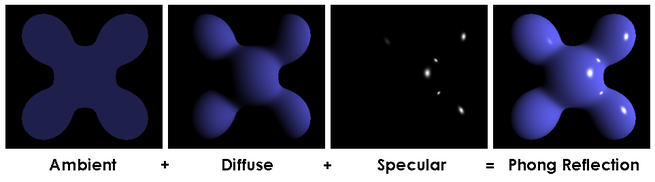
\includegraphics[scale=0.69]{./images/Phong_components_version_4.png}
        \caption{Visualisering af hhv. ambient, diffuse og speculars inflydelse på farven.}
    \end{figure}

    Alle lyskilder har 3 komponenter udover dets position:
    \begin{itemize}
        \item \(i_a\) er intensiteten for det omgivende lys.
        \item \(i_d\) er intensiteten for diffusen.
        \item \(i_s\) er intensitetn for spejlingen.
    \end{itemize}

    Intensiteten for det omgivende lys beregnes ofte ved at lægge værdierne for de forskellige lyskilder sammen.

    For hvert materiale er defineret:
    \begin{itemize}
        \item \(k_s\), der er en spejlingens refleksionskonstant.
        \item \(k_s\), der er diffuse reflektionskonstanten.
        \item \(k_a\), der er reflektionskonstanten for det omgivende lys.
        \item \(\alpha \), der er en konstant, der beskriver graden af glans.
    \end{itemize}

    Derudover er følgende defineret:
    \begin{itemize}
        \item \(objects\), der er en mængde af kugler. De bliver ikke brugt i formlen, men det er dem \(\hat{L_m} \ \textrm{og} \ \hat{N}\) afhænger af.
        \item \(lights\), der er en mængde af lyskilder.
        \item \(\hat{L_m}\), der er en retningsvektor fra punktet på objektet mod lyskilden.
        \item \(\hat{N}\), der er en normalvektor til punktet på objektet.
        \item \(\hat{R}\), der er den retning en perfekt reflekteret stråle ville tage.
              Den er udregnet således: \(\hat{R_m} = 2(\hat{L_m} \bullet \hat{N})\hat{N}-\hat{L_m})\)
        \item \(\hat{V}\), der er en retningsvektor, der beskriver hvilken vej kameraet peger.
    \end{itemize}

    Formlen beregner farven, \(I_p\) på et givent objekt. For simplicitets skyld antages det,
    at strålen altid rammer et af objekterne i scenen.

    \begin{equation}
        I_{p_n} = k_ai_a + \sum_{m \ \in \ lights}{k_d(\hat{L_m} \bullet \hat{N})\cdot i_{m,d} + k_s(\hat{R}_m \bullet \hat{V})^\alpha i_{m,s}} + I_{p_{n-1}}
    \end{equation}

    \section{Metoder}
    I programmering benyttes stepwise improvement til at skrive programmet. Der startes med at sende stråler gennem kameraet.
    Derefter findes der kugle-linje skæringspunkter. Til sidst implementeres Phong-reflektionsmodellen.
    Derudover er det skrevet funktionelt, altså det benytter det funktionelle paradigme med lambda funktioner
    og andre funktionelle koncepter.

    \section{Analyse}

    Programmet tager udgangspunkt i kugler, fordi de er den letteste ikke-trivielle form at tegne.

    \begin{figure}[H]
        \centering
        \begin{minted}[linenos]{text}
cast(ray, scene, depth, maxDepth):
    if depth is maxDepth return backgroundColor

    if not scene.intersect(ray):
        return backgroundColor
    
    [intersectionPoint, intersectionPointNormal] = scene.getIntersectionPoint(ray)
    reflectionRay = calculateReflectionRay(ray, intersectionPoint, intersectionPointNormal)
    reflectionColor = cast(reflectionRay, scene, depth + 1, maxDepth)

    ambientColor, diffuseColor, specularColor
    foreach light in scene.lights:
        lightDirection = normalize(light.position - intersectionPointNormal)
        viewDirection = normalize(ray.direction)

        ambientColor += light.ambient * material.ambient;

        diffuseIntensity = lightDirection.dot(intersectionPointNormal).max(0.0)
        diffuseColor += light.diffuse * (diffuseIntensity * material.diffuse)

        specularDirection = reflect(lightDirection, intersectionPointNormal)
        specularIntensity = specularDirection.dot(viewDirection).pow(material.shininess)
        specularColor += light.specular * (specularIntensity * material.specular)

    return ambientColor + diffuseColor + specularColor + reflectionColor

calculateReflectionRay(ray, intersectionPoint, intersectionPointNormal):
    reflectionDirection = reflect(ray.direction, intersectionPointNormal)
    return new Ray(intersectionPoint, reflectionDirection)
        \end{minted}
        \caption{Rekursiv Raytracing Algoritme (Pseudokode)}
    \end{figure}

    Først defineres cast funktionen.
    Den tager en lysstråle, scenen, nuværende dybde og max dybden den må rekursere, ind som argumenter.
    Scenen består af objekter, materialer og lyskilder,

    På linje 2 tjekkes om hvorvidt den skal rekursere videre, hvis ikke retunerer den baggrundsfarven.
    Derefter tjekkes om hvorvidt lysstrålen rammer nogen af objekterne i scenenm.
    Hvis ikke, retunerer den blot baggrundsfarven igen.

    Derefter beregnes refleksionsstrålen vha. calculateReflectionRay funktionen.
    Vi rekuserer ned og beregner reflektions farven.
    Derefter beregnes Phongs refleksionsmodel, hvorefter værdierne summes, som set i ligningen.
    Der afviges lidt fra modellen i den forstand, at der tjekkes om hvorvidt et objekt bliver ramt,
    mens der i modellen tages udgangspunkt i, at det gør den altid.

    Derudover summes værdierne for det omgivende lys også, hvilket heller ikke er set i modellen, men beskrevet i kilden.

    cast funktionen kaldes for hver pixel på skærmen, altså denne kan beskrives med \(width * height\).
    Dette betyder altså at den værste tidskompleksiteten er \(width*height*maxDepth+lights\), fordi der rekuserers ned maxDepth gange,
    hvor lights bliver itereret hver gang.

    \section{Perspektivering}

    Skulle projektet bygges igen, ville en langt mere optimal løsning involvere multithreading,
    enten på CPU'en eller med compute shaders eller på endnu mere dedikeret hardware som Nvidias RTX grafikkort.
    Dette ville resultere i at programmet kørte ca. 4-12x hurtigere afhængig af computeren programmet køres på.
    Derudover kunne det snildt køre 2000x hurtigere på GPU'en enten i form af compute shader
    \footnote{Programmer, der køres på GPU'en} eller cuda cores.\footnote{Specifikke kerner på RTX grafikkort}

    \section{Konklusion}

    Det kan konkluderes at raytracing er når det sendes stråler gennem et kamera ind i en 3D verden.
    hvorefter det med matematik, modelleres hvordan refleksioner og lys virker. Raytracing har positive egenskaber,
    der ikke findes ved konventionelle metoder som rasterisering. Derudover kan det konkluderes at det er en god måde at skabe realistiske verdener,
    dog er den meget tung at beregne, fordi dens tidskompleksitet er slem. Derudover bruger den mange tunge vektor operationer, der også tager tid at beregne.

    \newpage

    \section{Litteratur Liste}
    “1.2 Linjens Parameterfremstilling | MAT A Htx.” MAT A Htx, Systime, \url{https://mathtxa.systime.dk/?id=127}. Accessed 25 Feb. 2022.
    “5.5 Rekursion | MAT A Htx.” MAT A Htx, Systime,\url{ https://mathtxa.systime.dk/index.php?id=498&L=0}. Accessed 25 Feb. 2022.
    “---.” MAT A Htx, Systime, \url{https://mathtxa.systime.dk/?id=c2411&L=0}. Accessed 25 Feb. 2022.
    “---.” MAT A Htx, Systime, \url{https://mathtxa.systime.dk/index.php?id=498&L=0}. Accessed 25 Feb. 2022.
    Contributors to Wikimedia projects. “Phong Reflection Model - Wikipedia.” Wikipedia, the Free Encyclopedia, Wikimedia Foundation, Inc., 9 Jan. 2003, \url{https://en.wikipedia.org/wiki/Phong_reflection_model}.
    ---. “Pointer (Computer Programming) - Wikipedia.” Wikipedia, the Free Encyclopedia, Wikimedia Foundation, Inc., 30 Sept. 2001, \url{https://en.wikipedia.org/wiki/Pointer_(computer_programming)}.
    ---. “Ray Tracing (Graphics) - Wikipedia.” Wikipedia, the Free Encyclopedia, Wikimedia Foundation, Inc., 27 Sept. 2001, \url{https://en.wikipedia.org/wiki/Ray_tracing_(graphics)}.
    “Diskriminantformlen (Matematik B, Andengradspolynomium Og -Ligning) – Webmatematik.” Webmatematik, 8 Feb. 2011, \url{https://www.webmatematik.dk/lektioner/matematik-b/andengradspolynomium-og-ligning/diskriminantformlen}.
    “Kuglen (Matematik A, Vektorer i 3D) – Webmatematik.” Webmatematik, \url{https://www.webmatematik.dk/lektioner/matematik-a/vektorer-i-3d/kuglen}. Accessed 25 Feb. 2022.
    “Rekursive Funktioner.” People.Cs.Aau.Dk, Aarhus Universitet, \url{http://people.cs.aau.dk/~normark/c-prog-06/html/notes/functions_themes-rec-fu-sec.html}. Accessed 25 Feb. 2022.
    Rusty, Let’s Get. C++ RAII vs Rust OBRM - Part 2. YouTube, 23 Feb. 2022, \url{https://www.youtube.com/watch?v=7EcNkr6KFy0}.
    Wikimedia-projekter, Bidragsydere. “Vektor (Geometri) - Wikipedia, Den Frie Encyklopædi.” Wikipedia, Den Frie Encyklopædi, Wikimedia Foundation, Inc., 22 Apr. 2004, \url{https://da.wikipedia.org/wiki/Vektor_(geometri)}.


\end{flushleft}
\end{document}
